\documentclass[letterpaper,12pt]{article}
\usepackage{tabularx} % extra features for tabular environment
\usepackage{amsmath}  % improve math presentation
\usepackage{graphicx} % takes care of graphic including machinery
\usepackage[margin=1in,letterpaper]{geometry} % decreases margins
\usepackage{cite} % takes care of citations
\usepackage[final]{hyperref} % adds hyper links inside the generated pdf file
\hypersetup{
	colorlinks=true,       % false: boxed links; true: colored links
	linkcolor=black,        % color of internal links
	citecolor=blue,        % color of links to bibliography
	filecolor=magenta,     % color of file links
	urlcolor=blue         
}
\usepackage{blindtext}

%%%%%%%%%%%%%%%%%%%%%%%%%%%%%%%%%%%%%%%%%%%%%%%%%%%%%%%%%%%%%%%%%%%%%%%%%%%%%%%%%%%%%%%

% MY PACKAGES

% smart par skip
\usepackage{parskip}

% used to create cute quote 
\usepackage{csquotes}

% fix annoying positioning
\usepackage{float}

% cute tables
\usepackage{booktabs}

% testo intorno a figure
\usepackage{wrapfig, blindtext}

% used to highlight stuff
\usepackage{color,soul}

% MORE MATH
\usepackage{amsfonts}
\usepackage{amsmath}
\usepackage{amssymb}
\usepackage{mathrsfs}

% line breaks in cells
\usepackage{makecell, boldline}

%%%%%%%%%%%%%%%%%%%%%%%%%%%%%%%%%%%%%%%%%%%%%%%%%%%%%%%%%%%%%%%%%%%%%%%%%%%%%%%%%%%%%%%

% CUSTOM SETTINGS

\setlength\parindent{0pt}

% IMAGES SHORTCUT
\graphicspath{ {./images/} }

% INLINE CODE TEXT
\definecolor{codegray}{gray}{0.9}
\newcommand{\code}[1]{\colorbox{codegray}{\texttt{#1}}}

% CUSTOM LINESPREAD
\linespread{1.05}

% FAST CENTERED IMAGE
\newcommand{\imgc}[3]{\begin{figure}[H] 
  \centering
  \includegraphics[width=#1]{#2}
  \caption{#3}
\end{figure}}

% FIX CAPTION SPACE
\usepackage[font=small,skip=0.25cm]{caption}
\setlength{\belowcaptionskip}{-0.25cm}

% custom line width
\makeatletter
\def\thickhline{%
  \noalign{\ifnum0=`}\fi\hrule \@height \thickarrayrulewidth \futurelet
   \reserved@a\@xthickhline}
\def\@xthickhline{\ifx\reserved@a\thickhline
               \vskip\doublerulesep
               \vskip-\thickarrayrulewidth
             \fi
      \ifnum0=`{\fi}}
\makeatother

% custom citations
\usepackage{cite}

%%%%%%%%%%%%%%%%%%%%%%%%%%%%%%%%%%%%%%%%%%%%%%%%%%%%%%%%%%%%%%%%%%%%%%%%%%%%%%%%%%%%%%%

% CUSTOM PYTHON CODE

\usepackage{listings}
\usepackage{xcolor}

\definecolor{codegreen}{rgb}{0,0.6,0}
\definecolor{codegray}{rgb}{0.5,0.5,0.5}
\definecolor{codepurple}{rgb}{0.58,0,0.82}
\definecolor{backcolour}{rgb}{0.95,0.95,0.92}

\lstdefinestyle{mystyle}{
    backgroundcolor=\color{backcolour},   
    commentstyle=\color{codegreen},
    keywordstyle=\color{magenta},
    numberstyle=\tiny\color{codegray},
    stringstyle=\color{codepurple},
    basicstyle=\ttfamily\footnotesize,
    breakatwhitespace=false,         
    breaklines=true,                 
    captionpos=b,                    
    keepspaces=true,                 
    numbers=left,                    
    numbersep=5pt,                  
    showspaces=false,                
    showstringspaces=false,
    showtabs=false,                  
    tabsize=2
}

\lstset{style=mystyle}

%%%%%%%%%%%%%%%%%%%%%%%%%%%%%%%%%%%%%%%%%%%%%%%%%%%%%%%%%%%%%%%%%%%%%%%%%%%%%%%%%%%%%%%

\begin{document}

\title{\textbf{Network and Practical}}
\author{\textbf{Introduction to Machine Learning for Natural Language Processing}\\ \\ Daniele Passabì [221229], Data Science\\}

\date{\textit{\\Multi-class Classification of European Laws in Five Languages\\How do Recurrent Neural Networks Behave?}}
\maketitle
\thispagestyle{empty}

\begin{figure}[H] 
  \centering
  
\includegraphics[width=4cm]{logo.png}
\end{figure}

\newpage
\setcounter{tocdepth}{2}
\tableofcontents

\newpage
\clearpage
\pagenumbering{arabic}

%%%%%%%%%%%%%%%%%%%%%%%%%%%%%%%%%%%%%%%%%%%%%%%%%%%%%%%%%%%%%%%%%%%%%%%%%%%%%%%%%%%%%%%
% START HERE
%%%%%%%%%%%%%%%%%%%%%%%%%%%%%%%%%%%%%%%%%%%%%%%%%%%%%%%%%%%%%%%%%%%%%%%%%%%%%%%%%%%%%%%

%%%%%%%%%%%%%%%%
% INTRODUCTION %
%%%%%%%%%%%%%%%%

\section{Introduction}

Natural Language Processing (NLP) originated in the 1950s as the intersection of
artificial intelligence and linguistics \cite{nadkarni2011natural}. It arose in response to the many challenges presented by natural language.

The ambiguity of human language makes it extremely difficult to write software that accurately determines the meaning of text or speech data. Creating hand-written algorithms and rules that can work on any text is very complex, given the presence of homonyms, homophones, sarcasm, unspoken content, idioms, metaphors, grammar and usage exceptions in virtually any text.

NLP combines computational linguistics with statistical models and machine learning in order to successfully process human language in the form of text or speech, understanding its meaning in ways that traditional algorithms are unable to do \cite{IBM_NLP}.

Natural Language Processing is used to solve a wide range of tasks: in the following paper we are interested in the one of multi-class text classification. Furthermore, our attention will be drawn to a particularly problematic aspect of the NLP field: the fact that most algorithms are designed and implemented for only 7 of the more than 7000 languages spoken in the world. These are English, Chinese, Urdu, Farsi, Arabic, French, and Spanish \cite{TDS_NLP}.

Our objective aims to test whether different languages can influence architectures such as neural networks or statistical models. To this end, we used a dataset containing 65000 European laws, officially translated into several languages, on which we were able to compare the behaviour of various architectures, both with regard to fine-tuning and their performance.

The project code is public and available on \href{https://github.com/DanielePassabi/Uni_NLP2022_Exam}{Github}.
 


%%%%%%%%
% DATA %
%%%%%%%%
\newpage
\section{Data}

The chosen dataset, available on \href{https://huggingface.co/datasets/multi_eurlex}{HuggingFace}, comprises 65000 European laws officially translated into 23 languages. 

Of these available languages, five were selected, based on their adoption at European level:

\begin{itemize}
  \itemsep-0.3em
  \item \textit{English}, with 51\% EU speakers
  \item \textit{German}, with 32\% EU speakers
  \item \textit{Italian}, with 16\% EU speakers
  \item \textit{Polish}, with 9\% EU speakers
  \item \textit{Swedish}, with 3\% EU speakers
\end{itemize}


For each text in the dataset, there are one or more labels annotated. However, as can be understood by reading the paper on the dataset, these annotations are \textit{granular} \cite{Chalkidis2021MultiEURLEXA}. This allowed us to keep only the first level of labels, transforming the problem from a multi-label task to a multi-class one. This operation both simplified the problem and facilitated the evaluation of the architectures results.

This resulted in 21 different classes being initially present, shown in Figure \ref{fig:original_classes} together with the number of occurrences (texts) available for each of them.

\begin{figure}[H]
  \centering
  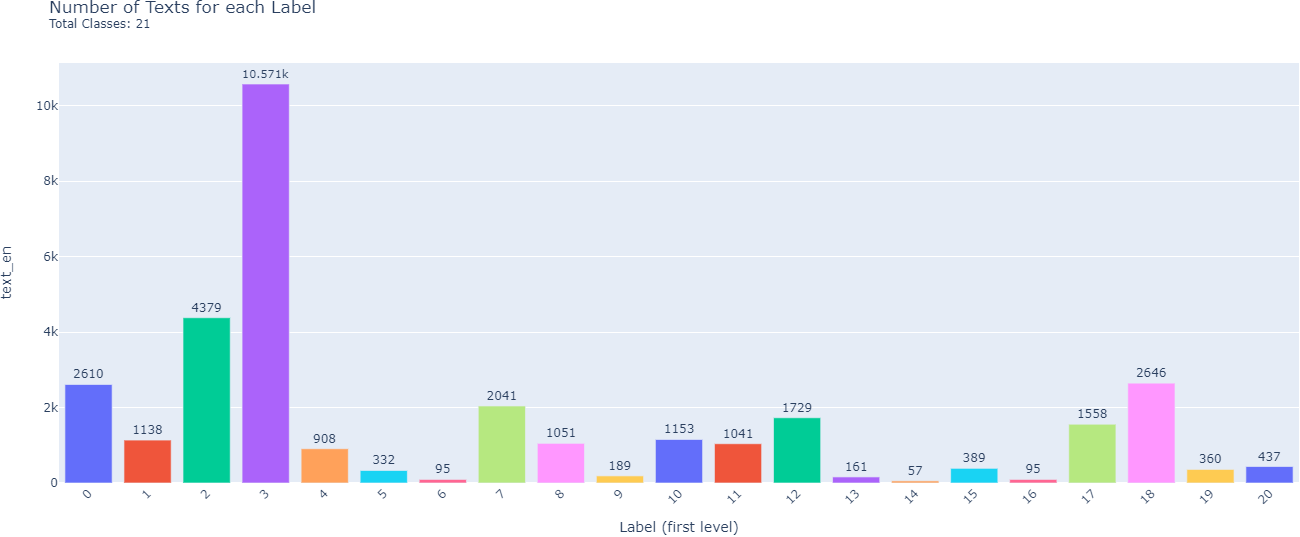
\includegraphics[width=\textwidth]{data_original_classes.png}
  \caption{MultiEURLEX Dataset - Distribution of Classes and Texts Occurrences}
  \label{fig:original_classes}
\end{figure}


A preliminary analysis of the data, however, revealed that each law averaged around 1200 words, with slight fluctuations depending on the considered language. Being aware that this factor would be computationally burdensome during the training phase of the models, it was decided to choose 2000 random laws from the three classes with the most observations, i.e. class 2, 3 and 18.

Ultimately, the final dataset consists of 6000 laws, officially translated into 5 languages and belonging to 3 distinct classes.

%%%%%%%%%
% MODEL %
%%%%%%%%%
\newpage
\section{Model}

In order to test the impact of different languages, various architectures were chosen, belonging both to the world of neural networks and statistics:

\begin{itemize}
  \item \textit{Long Short Term Memory}
  \item \textit{Convolutional Neural Network}
  \item \textit{Linear Support Vector Classifier}
\end{itemize}

\textit{TODO: DESCRIVERE LE ARCHITETTURE} 

%%%%%%%%%%%%%%%%%%%%%%
% EXPERIMENTAL SETUP %
%%%%%%%%%%%%%%%%%%%%%%
\newpage
\section{Experimental Setup}

\subsection{Data Cleaning and Preprocessing}

\subsection{Feature Extraction}

\subsection{Implementing the Architectures}

\subsection{Training Regime}



%%%%%%%%%%%
% RESULTS %
%%%%%%%%%%%
\newpage
\section{Results}



%%%%%%%%%%%%%%
% DISCUSSION %
%%%%%%%%%%%%%%
\newpage
\section{Discussion}



%%%%%%%%%%%%%%%%
% BIBLIOGRAPHY %
%%%%%%%%%%%%%%%%

% add bib to TOC
\addcontentsline{toc}{section}{Bibliography}

\newpage
\bibliographystyle{plain}
\bibliography{biblio} 

%%%%%%%%%%%%%%%%%%%%%%%%%%%%%%%%%%%%%%%%%%%%%%%%%%%%%%%%%%%%%%%%%%%%%%%%%%%%%%%%%%%%%%%

\end{document}
